\chapter{Experiments}

In the experimental phase, we selected datasets that have previously been utilized in well-recognized competitions. This allows us to benchmark the 
performance of our model against established baselines and leading-edge results within the field, helping us make meaningful comparisons with our model. 
Each dataset employed in our experiments represents a common scenario in the field of object detection, encompassing diverse environments and perspective 
urban life captured through ground-level cameras, aerial views provided by drones, and wide-ranging perspectives from satellites. 

\section{Datasets}
For the benchmarking of our model we decided to use three very well known datasets, and we are going to analyze in this section.


\subsection{Microsoft Common Object in COntext (MS COCO)}
The Microsoft Common Objects in Context (MS COCO) dataset 2017 is a comprehensive image dataset designed for object detection, segmentation, and captioning tasks. 
It is known for its complexity of its images, which are primarily sourced from everyday scenes. The dataset includes 80 object categories, providing a wide 
range of common objects for robust training and evaluation of machine learning models. These categories encompass various items from person, bicycle, 
car, to stop sign and smaller objects like toothbrush.

In terms of its composition, the MS COCO 2017 dataset contains over 118,000 training images, 5,000 validation images, and a test set of around 41,000 images, 
bringing its total to approximately 164,000 images. This dataset is also accompanied by over 1.5 million object instances, each annotated. 
The annotations are formatted to support both object detection and instance segmentation tasks. Specifically, for object detection, each annotation includes 
not only the class label and a bounding box defined by the $x$ and $y$ coordinates of the top-left corner, width, and height, but also a detailed segmentation 
mask for each object instance, making it suitable for more granular segmentation tasks as well.

The dataset is divided into training, validation, and test splits to facilitate the training and fine-tuning of models in a structured manner. 
This split ensures that models can be trained on a large set of images and parameters can be fine-tuned on the validation set before final evaluations 
are performed on the test set. The use of MS COCO for competition and research has helped advance the field of computer vision by providing a challenging 
set of images and annotations that test the limits of both existing and novel visual recognition models.

Class Distribution in COCO 2017:

\begin{figure}[h!]
    \centering
    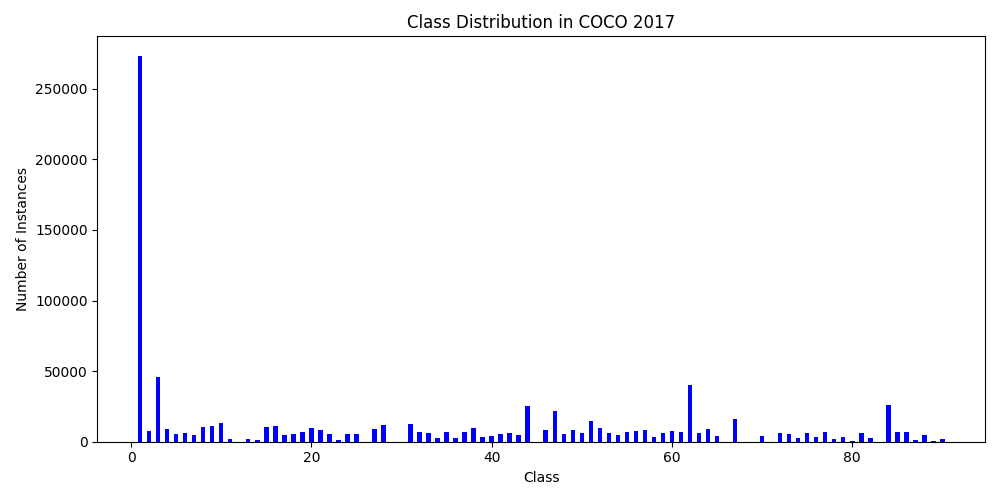
\includegraphics[scale=0.55]{Figures/coco2017_class_distribution.png}
    \caption{Class Distribution in COCO 2017}
    \label{fig:coco-class}
\end{figure}

\subsection{Unmanned Aerial Vehicle Small Object Detection}

The UAV-SOD (Unmanned Aerial Vehicle Small Object Detection) dataset is specifically designed for advancing research in the area of object detection using 
aerial imagery captured by drones. This dataset focuses on the detection of small objects, which presents unique challenges due to the small scale and often 
complex backgrounds seen in aerial images. Here are the key details about the UAV-SOD dataset. The UAV-SOD dataset includes detailed annotations for each image, 
essential for supervised machine learning models such as object detectors. Annotations are provided in XML format compatible with the PASCAL VOC annotation 
format, which is widely used in object detection tasks. These annotations include bounding boxes that specify the coordinates of each object in the image. 
The objects in this dataset are annotated with their class labels, enabling not only object detection tasks but also potential use for object classification 
and segmentation challenges.

Class Distribution in UAV Small Object Detection:

\begin{figure}[h!]
    \centering
    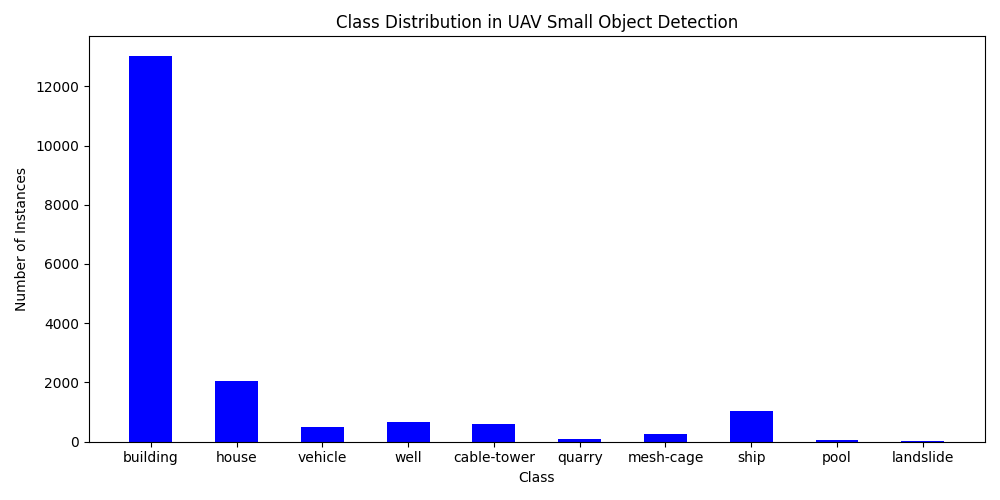
\includegraphics[scale=0.55]{Figures/uav_sod_data_class_distribution.png}
    \caption{Class Distribution in UAV Small Object Detection}
    \label{fig:uav-class}
\end{figure}


\subsection{VisDrone}

VisDrone is a dataset designed for drone-based object detection, featuring $10,209$ images captured across various environments using different 
types of drones. Each image in the dataset has a high resolution of $2000 \times 1500$ pixels. The dataset is organized into splits for comprehensive 
training and evaluation, consisting of $6,471$ images for training, $548$ images for validation, and $3,190$ images for testing. VisDrone includes a 
diverse set of ten object classes, such as pedestrians, cars, vans, buses, trucks, motorcycles, bicycles, awning-tricycles, and tricycles. This wide 
range of categories, combined with the diverse aerial perspectives provided by drone capture, makes VisDrone an ideal resource for developing and 
benchmarking deep learning models focused on enhancing object detection capabilities in drone surveillance systems.

Class Distribution in VIS Drone:

\begin{figure}[h!]
    \centering
    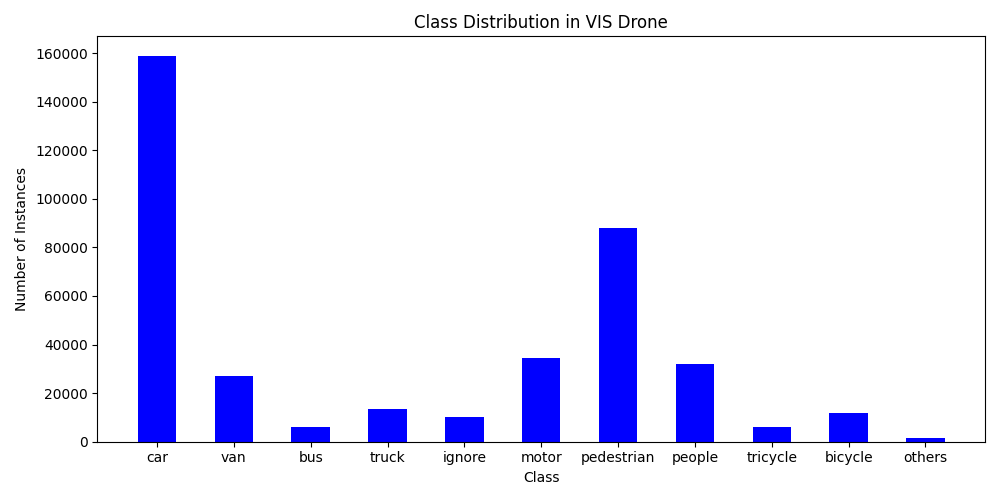
\includegraphics[scale=0.55]{Figures/vis_drone_data_class_distribution.png}
    \caption{Class Distribution in VIS Drone }
    \label{fig:vis-class}
\end{figure}



As we can understand from the class distribution, we can understand that class imbalance is present in the datasets. Class imbalance poses a significant 
challenge in training because models trained on such data may develop a bias towards more common classes and perform poorly on rare classes. 
We have to take this into consideration when choosing the evaluation metrics that give a more nuanced view of class-specific performance, such as 
per-class accuracy or the F1-score, are crucial for assessing a model’s true effectiveness across the varied classes present in these datasets.



\newpage
\section{Data Pre-Processing}

To ensure that the object detection models are trained on well-structured and uniform data, pre-processing steps are applied to standardize and enhance the 
raw dataset inputs. This process is crucial for achieving optimal model performance and is applied consistently across different datasets, such as COCO2017, 
UAV-SOD Drone, and Vis-Drone datasets, with specific adjustments tailored to each dataset's unique characteristics.

Firstly we have some general pre-processing steps applied across all datasets in order to make the training procedure 

\begin{enumerate}
    \item Resizing Images and Annotations: All images and corresponding annotations are resized to a uniform size of \(600 \times 600\) pixels. 
    This standardization helps maintain consistency across the dataset, which is crucial for the feature map creation with the Efficient-B7 model. 
    The resizing function also handles the segmentation data associated with each image, ensuring that all spatial information (bounding boxes and 
    segmentation masks) is correctly scaled and translated according to the new image dimensions.

    \item Image Padding: To maintain aspect ratio without distorting the image content, padding is applied using the most common color found in the image. 
    This approach prevents the introduction of biases that could occur if a non-representative color was used.

    \item Annotation Format: The annotation files for all the datasets have a common format in order to avoid any problems with the training process. The format 
    is the following: $x_{min}, y_{min}, x_{max}, y_{max}$, class code, $[(x_1, y_1), (x_2, y_2), ..., (x_n, y_n)]$, where the first four 
    values are the bounding box coordinates following the Pascal VOC format, then we have class code of the object and lastly the 
    list of coordinates describing the mask of the object.

    \item Mask Creation: The masks are a vital part of the model, since we want to use the functionality of the Masked-Attention Mask Transformer 
    in combination with the bounding box functionality to get better and more detailed results. The datasets ViS-Drone and 
    Unmanned Aerial Vehicle datasets do not include masks and in order to have mask data we generate masks from the bounding box 
    data. More specifically the mask data format is the following: \\
    $[(x_{min}, y_{min}), (x_{min}, y_{max}), (x_{max}, y_{min}), (x_{max}, y_{max})]$

    \item Calculation of Mean and Standard Deviation: For normalization purposes, the mean and standard deviation of the pixel values across the dataset are 
    computed. These statistics are essential for normalizing the images during the model training process, 
    allowing for faster convergence and improved generalization.

    \item Visualization of Data: Functions are included to plot images alongside their annotations for both training and validation sets. This visual check 
    allows for the verification of the correct processing and annotation of the data, ensuring integrity before training begins.

  \end{enumerate}



\newpage

Furthermore we make specific changes to each dataset in order to ensure compatibility with the model. These changes are:

\begin{enumerate}
    \item \textbf{COCO2017 Dataset - } Annotation Conversion: The original COCO annotations are converted into a simpler text format that includes bounding 
    box coordinates and segmentation data. This conversion facilitates the use of custom training pipelines that may not natively support COCO's complex 
    annotation format.

    \item \textbf{Vis-Drone Dataset - } Annotation Format Standardization: The annotations provided with the Vis-Drone dataset are standardized to ensure 
    consistency with other datasets. This process includes recalculating bounding box coordinates from $[x_{min}, y_{min}, width, height]$ to  
    $[(x_{min}, y_{min}), (x_{min}, y_{max}), (x_{max}, y_{min}), (x_{max}, y_{max})]$

    \item \textbf{UAV-SOD Drone Dataset - } XML to Text Conversion: Given that UAV-SOD annotations might be provided in XML format, a conversion process 
    is implemented to translate these XML files into a plain text format that is easier to manipulate and integrate into training workflows. The conversion 
    also involves mapping categorical names to predefined numerical codes, which are crucial for consistent label encoding across different datasets.
\end{enumerate}

These pre-processing steps are critical for preparing the data, ensuring that it meets the necessary format and quality standards required for effective 
model training. This comprehensive approach to data preparation helps in minimizing issues during training, leading to more robust and accurate object 
detection models.



\section{Evaluation Metrics}


Evaluation metrics are vital in object detection as they quantitatively measure a model's accuracy, robustness, and effectiveness in predicting correct 
object locations and classifications. These metrics enable developers to compare different models, optimize parameters, and ensure that the system performs 
well across various conditions and datasets, guiding improvements and ensuring that the deployed models meet the required performance standards. Starting 
with the basic definitions we have:

\begin{enumerate}
    \item True Positives (TP) are the predictions that correctly match the class of the ground truth AND Confidence and IoU scores are 
    higher than their thresholds.
    \item False Positive (FP) are the predictions that incorrectly predict a positive class when the ground truth is actually negative 
    OR the IoU score is lower than the threshold.
    \item False Negative (FN) occurs when the model misses positive instances. It predicts a negative class when the ground truth is actually positive.
    \item True Negative (TN) represents instances where the confidence score of a detection that is not supposed to detect anything is lower than 
    the threshold. This metric is not used in the object detection field since there are too many boxes that should not detect an object in an image.
\end{enumerate}


The metrics we are going to be using that are object detection specific are the Average Precision (AP), mean Average Precision (mAP), Intersection over 
Union (IoU), Average Recall (AR) and mean Average Recall (mAR). \\


Recall \cite{metrics} measures the proportion of actual positives that are correctly identified by the model, indicating the model’s ability to detect all relevant instances.
\begin{equation}
    \text{Recall} = \frac{TP}{TP + FN} \tag{16}
\end{equation}


Precision \cite{metrics} indicates the accuracy of the positive predictions made by the model, measuring the proportion of positive identifications that were actually correct.
\begin{equation}
    \text{Precision} = \frac{TP}{TP + FP} \tag{17}
\end{equation}

F1-Score \cite{metrics} is the harmonic mean of precision and recall, providing a balance between the two by penalizing extreme values.

\begin{equation}
    F1 = 2 \cdot \frac{\text{Precision} \times \text{Recall}}{\text{Precision} + \text{Recall}} \tag{18}
\end{equation}


Intersection Over Union (IoU) \cite{metrics} assesses the overlap between predicted bounding boxes and ground truth boxes, quantifying the exactness of the location 
of predictions. It is a fundamental metric for determining whether a detection is a true.

\begin{equation}
    IoU = \frac{\text{Area of Overlap}}{\text{Area of Union}} \tag{19}
\end{equation}


Average Precision (AP) \cite{metrics}quantifies the precision of an object detector across different recall levels by taking the mean of precisions computed 
at the point of each of the 11 recall levels. The precision at each recall level $r$ is interpolated by taking the maximum precision measured 
for a method at any recall level $\geqslant r$

\begin{equation}
    AP = \frac{1}{11} \sum_{r \in \{0.0, 0.1, \ldots, 1.0\}} P_{\text{interp}}(r) \tag{20}
\end{equation}


Mean Average Precision (mAP) \cite{metrics} is the average of the AP scores for all classes or over different Intersection over Union (IoU) thresholds. 
This metric gives an overall effectiveness of the detection model across various object categories or detection precisions, making it ideal for 
scenarios where multiple object types are involved.
\begin{equation}
    mAP = \frac{1}{N} \sum_{i=1}^{N} AP_i \tag{21}
\end{equation}


\newpage
\section{Training}

To implement the Extended Masked-Attention Mask Transformer, we utilized Amazon Web Services (AWS) SageMaker for efficient training and experimentation. 
Specifically, we employed the \textit{ml.p4d.24xlarge} instance type for our notebook environment, which is equipped with eight NVIDIA A100 GPUs and supports CUDA 12.1. 
This powerful computational setup allowed us to run the training with a batch size of four images per batch, achieving an optimal balance between convergence 
speed and model accuracy.

The weights of the network were initialized using the default settings provided by PyTorch, ensuring standard initialization practices. All experiments were 
conducted using this configuration to maintain consistency and reliability in our results. By leveraging the capabilities of AWS SageMaker and the high-performance 
computing resources of the \textit{ml.p4d.24xlarge} instance, we were able to efficiently train the model and effectively utilize the limited data from small objects in images.

To provide clarity on our training setup and ensure reproducibility, the table \ref{tab:training_parameters} summarizes the key training parameters used for the 
Extended Masked-Attention Mask Transformer. These parameters were carefully selected based on extensive experimentation to achieve an optimal balance between 
convergence speed and model accuracy. 
\begin{table}[h]
\centering
\begin{tabular}{|c|c|c|c|}
    \hline
    &                   \textbf{MS COCO}      & \textbf{UAV-SOD}     & \textbf{VisDrone}            \\ \hline
    Number of Epochs   & 125                  & 75                   & 75                           \\ \hline
    Optimizer          & AdamW                & AdamW                & AdamW                        \\ \hline
    Learning Rate      & $1 \times 10^{-4}$   & $1 \times 10^{-3}$   & $1 \times 10^{-3}$           \\ \hline
    Batch size         & 4                    &  4                   & 4                            \\ \hline
    Image size         & $600\times600$       &  $600\times600$      & $600\times600$               \\ \hline
    Number of Anchors  & $30000$              &  $722$               & $722$                        \\ \hline
\end{tabular}
\caption{Details of training parameters per dataset}
\label{tab:training_parameters}
\end{table}

\newpage

\section{Results}

Following the comprehensive description of our training setup and parameters, we now present the results of our experiments with the Extended Masked-Attention 
Mask Transformer. This section delves into the performance metrics achieved by the model, highlighting its effectiveness in both object detection and instance 
segmentation tasks. We evaluate the model's ability to accurately detect and segment objects of various sizes within images, with a particular focus on its 
performance on small objects, which pose significant challenges due to their limited visual information.


\subsection{Microsoft Common Object in COntext (MS COCO)}

\begin{table}[h]
    \centering
    \begin{tabular}{|c|c|c|c|}
        \hline
        \textbf{Model}     & \textbf{mAP(@0.5)}     & \textbf{mAP(@0.5:0.95)}  & \textbf{Parameters}   \\ \hline
        EMAMT              & 125                    & 75                       & 75                    \\ \hline
        MAMT               & 125                    & 75                       & 75                    \\ \hline
    \end{tabular}
    \caption{Results of training for COCO dataset}
    \label{tab:coco_results}
\end{table}



\subsection{Unmanned Aerial Vehicle Small Object Detection}
\begin{table}[h]
    \centering
    \begin{tabular}{|c|c|c|c|}
        \hline
        \textbf{Model}     & \textbf{mAP(@0.5)}     & \textbf{mAP(@0.5:0.95)}  & \textbf{Parameters}   \\ \hline
        EMAMT              & 125                    & 75                       & 75                    \\ \hline
        MAMT               & 125                    & 75                       & 75                    \\ \hline    
    \end{tabular}
    \caption{Results of training for UAV-SOD dataset}
    \label{tab:uav_results}
\end{table}





\subsection{VisDrone}
\begin{table}[h]
    \centering
    \begin{tabular}{|c|c|c|c|}
        \hline
        \textbf{Model}     & \textbf{mAP(@0.5)}     & \textbf{mAP(@0.5:0.95)}  & \textbf{Parameters}   \\ \hline
        EMAMT              & 125                    & 75                       & 75                    \\ \hline
        MAMT               & 125                    & 75                       & 75                    \\ \hline
    \end{tabular}
    \caption{Results of training for VisDrone dataset}
    \label{tab:vis_results}
\end{table}